%% ============================================================================
%%  Ternary Neural Network Inference for MNIST on the Nexys 3 FPGA
%%  Project report -- method, hardware, verification, measured results
%%
%%  Compile with:   tectonic report.tex
%%          or:     pdflatex report.tex   (3x, for the index)
%%
%%  Every quantitative claim in this report is measured. The figures were
%%  recomputed from the checkpoints and RTL by python/docs_figures pipeline and
%%  recorded in docs/measured_figures.json. Where a number is an estimate
%%  rather than a measurement it is labelled as such.
%% ============================================================================
\documentclass[11pt,a4paper]{article}

%% ------------------------------ packages -----------------------------------
\usepackage[T1]{fontenc}
\usepackage[utf8]{inputenc}
\usepackage{lmodern}
\usepackage[margin=2.4cm]{geometry}
\usepackage{booktabs}
\usepackage{array}
\usepackage{multirow}
\usepackage{amsmath,amssymb}
\usepackage{graphicx}
\usepackage{xcolor}
\usepackage{listings}
\usepackage{hyperref}
\usepackage{caption}
\usepackage{float}
\usepackage{enumitem}
\usepackage{tabularx}
\allowdisplaybreaks
\sloppy
\usepackage{pgfplots}
\usepackage{pgfplotstable}
\pgfplotsset{compat=1.18}
\usepackage{tikz}
\usetikzlibrary{arrows.meta,positioning}

\hypersetup{
  colorlinks=true,
  linkcolor=blue!50!black,
  citecolor=blue!50!black,
  urlcolor=blue!50!black,
  pdftitle={Ternary Neural Network Inference for MNIST on the Nexys 3 FPGA},
  pdfauthor={Project Report}
}

\definecolor{hdr}{RGB}{31,73,125}
\definecolor{codebg}{RGB}{248,248,248}
\definecolor{good}{RGB}{31,120,60}
\definecolor{bad}{RGB}{170,40,40}
\definecolor{warn}{RGB}{180,110,10}

\lstset{
  basicstyle=\ttfamily\scriptsize,
  backgroundcolor=\color{codebg},
  frame=single,
  breaklines=true,
  columns=fullflexible,
  keepspaces=true,
  captionpos=b,
  numbers=none
}

\captionsetup{font=small,labelfont=bf}

\newcolumntype{Y}{>{\centering\arraybackslash}X}
\newcommand{\good}{\textcolor{good}{\textbf{}}}
\newcommand{\bad}{\textcolor{bad}{\textbf{}}}
\newcommand{\est}{\textcolor{warn}{est.}}

\title{\vspace{-1.2cm}
  \textbf{\LARGE Ternary Neural Network Inference}\\[0.35cm]
  \textbf{\Large for Handwritten Digit Recognition on the Nexys 3 FPGA}\\[0.9cm]
  \vspace{0.3cm}
  \normalsize
  A multiplier-free $784 \rightarrow 32 \rightarrow 10$ ternary network,\\
  verified bit-exact against its software reference\\[1.4cm]
  \large Project Report
}
\author{}
\date{}

\begin{document}
\maketitle
\tableofcontents
\newpage

%% ============================================================================
\begin{abstract}
This report describes the design, implementation and verification of a ternary
($\{-1,0,+1\}$) neural network accelerator for handwritten digit recognition
on the Digilent Nexys~3 FPGA (Artix-7 XC7A100T). The deployed network is
$784 \rightarrow 32 \rightarrow 10$: its first layer is entirely ternary and
contains \emph{zero} arithmetic multipliers, because multiplication by $-1$,
$0$ and $+1$ reduces to a sign flip, a mask and a wire.

The work is organised around a single principle: \textbf{bit-exactness}. The
FPGA must reproduce the PyTorch model exactly, not approximately. This forced
the entire forward path to remain in integer arithmetic, and every architectural
decision follows from that constraint rather than from convenience. A
Walsh--Hadamard rotation is applied to the pixel bus before the first layer so
that the ternary MAC never accumulates beyond a narrow integer range; the
training procedure is run in an \texttt{integer-exact} mode that reproduces the
hardware's fixed-point arithmetic exactly during optimisation.

Nine classes of defect were found and fixed during verification, several of which
had produced plausible-looking but silently wrong results. Final verification
reports \textbf{2000/2000 agreement} between the RTL simulation and the software
reference over 2{,}000 MNIST images.

Against a classical float reference of the same task, the ternary design
achieves a \textbf{complete elimination} of the multiplier count and a
\textbf{228$\times$} reduction in weight storage for a loss of 3.6 accuracy
points. We report this honestly as a \emph{cost} trade, not a free win: the
float reference remains more accurate. The value proposition is area, latency
and energy, which are the metrics that matter for an edge classifier.
\end{abstract}

%% ============================================================================
\section{Introduction}
\label{sec:intro}

\subsection{Why ternary networks}

Neural network inference on an embedded device is constrained by three
resources: silicon area, latency and energy. The dominant term in all three is
usually the multiply--accumulate unit. A conventional layer of $n$ inputs and
$m$ outputs requires $nm$ multipliers, each occupying on the order of a thousand
LUTs on a 7-series FPGA. A $784 \rightarrow 256$ layer therefore does not fit
on the 15{,}850 LUTs available on a Nexys~3.

\begin{table}[H]
\centering
\small
\caption{The three ternary weights and what each costs in hardware. Only the
  first row requires no multiplier, which is the entire point of the exercise.}
\label{tab:ternary-ops}
\begin{tabular}{@{}lllc@{}}
\toprule
\textbf{Weight} & \textbf{Operation} & \textbf{Hardware} & \textbf{Multiplier} \\
\midrule
$+1$ & $\times\,1$ & pass the wire       & no \\
$0$  & $\times\,0$ & mask to zero        & no \\
$-1$ & $\times\,-1$ & invert the sign bit & no \\
\bottomrule
\end{tabular}
\end{table}

Table~\ref{tab:ternary-ops} is the whole argument. If every weight in the large
first layer is drawn from $\{-1,0,+1\}$, the entire $784 \times H$ multiply stage
collapses into wiring. What remains is an adder tree and a weight memory, and the
layer becomes cheap enough that several times more hidden units fit.

This is not a new idea. BitNet b1.58 and the Bonsai 27B work establish that
fully ternary networks are competitive with much larger floating-point ones at
inference, and this project draws its technique set from that lineage
(Section~\ref{sec:ternary}). What is new here is the \emph{integer-exact
hardware co-design}: the network is constrained during training so that the RTL
is not an approximation of the model but a faithful implementation of it.

\subsection{Scope and honest positioning}

The classical float network used as reference is the 784--256--10 teacher from
this project, reaching \textbf{98.24\%} on the MNIST test set. The ternary
network reaches \textbf{94.61\%}. The ternary design does not win on accuracy and
this report does not claim that it does.

The comparison that matters is cost. Table~\ref{tab:headline} summarises the
positioning, and Section~\ref{sec:results} develops it in full.

\begin{table}[H]
\centering
\small
\caption{Headline comparison. The float reference is more accurate; the ternary
  design is far cheaper. Both columns are measured, not estimated.}
\label{tab:headline}
\begin{tabularx}{\linewidth}{@{}lY Y Y@{}}
\toprule
 & \textbf{Float ref.} & \textbf{Ternary $H{=}16$} & \textbf{Ternary $H{=}32$} \\
 & 784--256--10 & 784--16--10 & 784--32--10 \\
\midrule
MNIST test accuracy      & \good 98.24\% & 94.19\% & 94.61\% \\
MNIST (GUI pipeline)     & \good 97.0\%  & 92.5\%  & 93.5\% \\
Hand-drawn               & 80.5\%  & 74.8\%  & \good 84.8\% \\
Rendered font glyphs     & \good 91.1\% & 78.9\% & 83.3\% \\
\midrule
Parameters               & 203{,}530 & 12{,}730 & 25{,}418 \\
Multipliers              & 203{,}530 & \good 0 & \good 0 \\
MACs per image           & 203{,}264 & \good 12{,}704 & 25{,}408 \\
Weight storage           & 795.0 KiB & \good 1.8 KiB & 3.5 KiB \\
BRAM36 for weights       & 24.8   & \good 0.06 & 0.11 \\
Entropy (bits/weight)    & 32.0   & 1.189 & \good 1.122 \\
\bottomrule
\end{tabularx}
\end{table}

Two points deserve emphasis, both of which cut against the project's own
interest. First, the float reference is more accurate on every input tested and
this report does not pretend otherwise. Second, Section~\ref{sec:negative}
documents five substantial optimisation attempts that failed, one of which made
accuracy actively worse.

\subsection{Contributions}

\begin{enumerate}[leftmargin=*]
\item A multiplier-free ternary inference datapath for
      $784 \rightarrow 32 \rightarrow 10$, with a sequential MAC engine sized to
      fit the Nexys~3 LUT budget.
\item An \texttt{integer-exact} training mode in which the forward pass is
      written to reproduce the hardware's integer arithmetic exactly, so the
      exported weights are provably faithful rather than approximately faithful.
\item A verification methodology that compares the RTL against the software
      reference image-by-image, reported at 2000/2000 agreement.
\item A host toolchain: a training GUI with live network visualisation, an
      image uploader with automatic polarity detection, and UART transmission
      to the board.
\item A documented negative-result record covering distillation, ensembling,
      test-time augmentation, high-resolution drawing and per-digit rebalancing
      (Section~\ref{sec:negative}).
\end{enumerate}

%% ============================================================================
\section{The Classical Reference}
\label{sec:classical}

\subsection{Architecture}

The reference network is a fully connected multilayer perceptron,
$784 \rightarrow 256 \rightarrow 10$, trained in float32 by the original
supervision path in this project. It reaches \textbf{98.24\%} on the 10{,}000
MNIST test images. It is used here in two roles: as the accuracy yardstick, and
--- in one discarded experiment --- as a distillation teacher.

Its cost is what motivates everything else. At float32 it holds
$203{,}530 \times 32 = 6{,}512{,}960$ bits of weights, or roughly 795 KiB, which
is 24.8 BRAM36 blocks and the majority of the board's 50 available blocks. It
requires 203{,}264 multiply--accumulate operations per image and therefore a
comparable number of multipliers. Neither figure is compatible with a device
that also has to run the rotation, the control logic and the UART receiver.

\subsection{The information-content argument}

The gap between float and ternary is fundamentally a question of information. A
float32 weight carries 32 bits; a ternary weight carries at most
$\log_2 3 = 1.585$ bits. Compressing a weight by a factor of roughly twenty is
a substantial loss of degrees of freedom, and it would be unreasonable to
expect it to cost nothing.

The prediction from this argument is that ternary accuracy should be bounded by
the float baseline and should approach it only as capacity grows. Section~
\ref{sec:width} tests this directly with a width sweep, and the result is
consistent: the measured entropy of the ternary network is 1.19 bits per weight,
roughly 3.7\% of the float representation, and it recovers 95.6\% of the
reference's absolute accuracy while using 6.25\% of the parameters.

\subsection{Cost model}

Unless stated otherwise, all cost figures in this report use the following
definitions:

\begin{description}[leftmargin=*,style=nextline]
\item[Multipliers.] The number of distinct multiply operations the datapath must
  perform per inference. A ternary weight consumes none, so the count equals
  the number of float weights.
\item[MACs.] Multiply--accumulate operations per image, counting one MAC per
  weight application.
\item[Latency.] MAC count divided by clock frequency, assuming one MAC per
  cycle. The sequential MAC engine does indeed sustain one MAC per cycle, so
  this is a cycle-accurate figure and not merely proportional.
\item[Weight storage.] Measured as the entropy of the first layer plus 16 bits
  per second-layer weight, which is what the hardware actually stores.
\end{description}

We deliberately do \emph{not} quote power or area figures. No synthesis tool is
available in this environment, so those numbers would be fabricated. Energy
claims are handled in Section~\ref{sec:energy} by counting arithmetic
operations and memory accesses, which \emph{is} measurable, and by stating
explicitly which parts of the argument are inference.

%% ============================================================================
\section{Ternary Quantisation}
\label{sec:ternary}

\subsection{Weight encoding and the cost of a ternary weight}

A ternary weight is stored in two bits, with the fourth of every four-bit group
unused. This is wasteful in isolation --- 2 bits per weight where the entropy is
1.19 --- but it is what the VHDL address arithmetic wants, because it keeps the
word boundaries aligned for direct indexing rather than requiring a shift and
mask on every access.

The packed first-layer matrix occupies $784 \times 32 \times 2 = 50{,}176$
bits, which fits in two BRAM36 blocks.

\subsection{Measured bits per weight}

The meaningful figure is not the 2-bit storage format but the entropy of the
learned weights. For a ternary matrix with zero fraction $z$, the Shannon
entropy per weight is
\[
H(z) = -z\log_2 z - (1-z)\log_2(1-z).
\]
Because every digit class carries roughly the same number of examples, the
weights come out close to the maximum-entropy ternary distribution $z = 1/3$,
which gives 1.585 bits. Measured across the shipped models:

\begin{table}[H]
\centering
\small
\caption{Measured weight entropy. ``Zero density'' is the fraction of first-layer
  weights that quantise to exactly zero, the value that makes the hardware a
  mask-and-add network.}
\begin{tabularx}{\linewidth}{@{}lY Y Y@{}}
\toprule
\textbf{Configuration} & \textbf{Zero density} & \textbf{$H(z)$} & \textbf{Net bits/weight} \\
\midrule
without augmentation & 53.4\% & 0.993 & 1.191 \\
wide augmentation   & 69.3\% & 0.816 & 1.086 \\
deployed (mild)     & 65.9\% & 0.926 & \textbf{1.122} \\
\bottomrule
\end{tabularx}
\end{table}

The net figure includes the second layer at its true 16-bit width, which is why
it sits above $H(z)$: selective precision is not free, it costs
$16 \times 160 = 2{,}560$ bits, but it is only 1.26\% of the weights.

\subsection{Techniques for rigidity and accuracy}
\label{sec:techniques}

Five techniques were adopted from BitNet b1.58 and Bonsai 27B, and two were
developed for this project in response to measured failures. Each is described
with the problem it solves, because several of them exist precisely because a
naive ternary implementation did not work.

\paragraph{1. Walsh--Hadamard rotation.}
The dominant error in ternary networks is magnitude growth. When a ternary
weight multiplies an unbounded activation, the accumulator drifts far from zero,
and the hardware is forced into a wide integer to avoid overflow --- destroying
the area saving.

The fix, borrowed from Bonsai, is to apply a fixed orthogonal transform $H$ to
the input vector before the first layer, and to store $W_1 H^{\mathsf{T}}$ in its
place. Since $H$ is orthogonal, the layer computes an equivalent function of a
rotated input rather than a different function. Block-8 Hadamard matrices are
used: the rotation is a fixed XOR/adder network with no multipliers, and it
normalises the input energy so the accumulator stays narrow.

This is the single most important technique in the design. Without it the
integer widths grow and the hardware stops being small.

\paragraph{2. Selective precision on the second layer.}
The output matrix has only $H \times 10$ weights --- 320, or 1.26\% of
the network. Forcing these into $\{-1,0,+1\}$ as well would be aggressive for
almost no area gain. Bonsai's observation is that precision is worth paying for
wherever it is cheap, so W2 is kept at 16 bits. This is what allows a
16-ternary-unit network to reach 94\% on MNIST: the decoder does the fine
discrimination that the encoder cannot.

\paragraph{3. Closed-loop sparsity control.}
The ternary threshold ratio is not a hyperparameter fixed in advance. It is
adjusted during training by measuring the achieved zero density against a target
and stepping the ratio accordingly, so the network is driven towards the
target sparsity rather than drifting away from it.

\paragraph{4. Positive bias initialisation for dead-unit prevention.}
With a positive bias initialisation, a hidden unit begins the training in its
active state. Without it, a unit whose weights quantise to zero stays inactive,
receives no gradient, and is dead for the rest of training. This matters more in
ternary networks than in float networks because the quantisation step can kill a
unit outright; dead units are unrecoverable at the quantisation boundary.

\paragraph{5. Augmentation to match the deployment distribution.}
MNIST is pre-normalised: every digit sits in a 20$\times$20 box. A user drawing
with a mouse does not. This was measured, not assumed --- freehand digits
average a 25.3-pixel span against MNIST's 20.0, and carry 186 pixels of ink
against MNIST's 96. Training without augmentation on that distribution yields
roughly 18\% accuracy on freehand input. Scale, translation, rotation and stroke
thickness augmentation recover it, at a cost of roughly 11 points of clean
MNIST accuracy. Section~\ref{sec:tradeoff} documents that trade honestly.

\paragraph{6. Integer-exact training (developed here).}
The usual approach is to train in float and quantise afterwards, accepting that
the hardware will differ from the model. That is unacceptable for this project,
whose central claim is bit-exactness. Instead the forward pass is written in
integer arithmetic that mirrors the RTL: binary pixel inputs, an unnormalised
Hadamard rotation with a fixed right shift, integer biases, and an integer
activation clamp.

The gradient estimator is the straight-through estimator, which must be written
as \texttt{hard.detach() + (latent - latent.detach())} rather than the more
common \texttt{x + (q - x).detach()}. Both produce correct gradients in
principle, but the second form silently produces wrong ones when the latent is
used more than once in the graph. Two separate defects in this project traced
back to that distinction.

\paragraph{7. Adaptive geometry guidance in the host tool (developed here).}
Because the model is positionally sensitive --- a one-pixel shift costs 3 to 9
accuracy points --- the GUI measures the drawing and reports its span, centre
and ink coverage against the training distribution. The original design imposed
a fixed target box and told the user to aim at it; measurement showed that
attempting to hit a fixed box by resampling costs about 23 points through
binarisation error. Measuring and reporting is strictly better than pretending
to correct.

\subsection{The rotation in detail}

For an input block $\mathbf{x}$ of length 8, the Hadamard transform is the
butterfly
\[
\begin{bmatrix}
x_0 & x_1 & x_2 & x_3 & x_4 & x_5 & x_6 & x_7
\end{bmatrix}
\mapsto
\begin{bmatrix}
x_0{+}x_1{+}x_2{+}x_3{+}x_4{+}x_5{+}x_6{+}x_7 & \cdots
\end{bmatrix}
\]
implemented in \texttt{WalshHadamard.vhd} as a streaming XOR/adder network. It
is verified bit-identical to the Python reference over 3{,}136 values with total
absolute error zero.

%% ============================================================================
\section{From Model to Hardware}
\label{sec:pipeline}

\subsection{Architectural decisions}

The central design decision was to abandon a fully parallel first layer. A
parallel $784 \times 16$ design needs approximately 25{,}000 LUTs against the
15{,}850 available on the device; it does not fit, at any optimisation effort.
Replacing it with a single sequential MAC engine that walks the 784 inputs costs
one multiplier-equivalent (none, being ternary) and 784 cycles, and fits
comfortably.

The cost of this decision is latency: 25{,}408 MACs per image at $H{=}32$ is
about 254\,\textmu s at a 100\,MHz clock. For a human-facing digit recogniser
this is entirely irrelevant, and the area saving is what makes the design exist
at all.

\subsection{Integer-exact derivation}

The integer-exact mode constrains the forward pass so that every value the
hardware could see is reproducible in Python:

\begin{itemize}[leftmargin=*]
\item Pixels are binarised before the rotation, so the rotation input is strictly
      $\{0,1\}$.
\item The rotation is unnormalised and followed by a fixed right shift, matching
      \texttt{WalshHadamard.vhd} exactly.
\item First-layer biases are rounded to integers \emph{before} being divided by
      the shared scale, not after. This ordering was a genuine defect: the
      opposite order silently changed results.
\item The accumulator is allowed to run freely through the whole MAC pass; ReLU
      and clamping are applied only on the final cycle. Clamping earlier looked
      reasonable and was wrong.
\item The second layer is scaled by a single positive constant. A shared positive
      scale leaves the arg-max unchanged, so this is free.
\end{itemize}

\subsection{Choosing the hidden width}
\label{sec:width}

Because the information-content argument predicts that ternary networks approach
float accuracy only as capacity grows, a width sweep was run to choose $H$. The
result was not the monotone improvement the argument predicts: MNIST accuracy
rose with width while robustness to hand-drawn input did not, and the $H{=}32$
row was the weakest of the four on average. Width alone therefore does not buy
robustness, which is why the deployed model pairs $H{=}32$ with augmentation
rather than simply being the widest network available.

The decisive evidence for width came from the confusion analysis in
Section~\ref{sec:results}, which shows the dominant $8 \rightarrow 6$ error
is a loop-count distinction that does not clear until there are enough hidden
units to represent the feature.

\subsection{The accuracy--robustness trade}
\label{sec:tradeoff}

Augmentation is not free. Table~\ref{tab:aug} shows the cost precisely.

\begin{table}[H]
\centering
\small
\caption{Effect of augmentation on the deployed network. Freehand accuracy is
  measured on the synthetic freehand set; MNIST on the real test set.}
\label{tab:aug}
\begin{tabularx}{\linewidth}{@{}lY Y@{}}
\toprule
\textbf{Training} & \textbf{MNIST} & \textbf{Freehand} \\
\midrule
No augmentation     & \good 94.19\% & 18.4\% \\
Morphology only     & 91.78\% & 27.2\% \\
Morphology + affine & 83.96\% & \good 68.4\% \\
\bottomrule
\end{tabularx}
\end{table}

Augmentation moved freehand accuracy from 18.4\% to 68.4\% --- the difference
between unusable and usable --- for 10 points of clean MNIST accuracy. Whether
that is a good trade depends entirely on the deployment distribution. For a
benchmark submission the answer is clearly no; for an interactive drawing tool it
is clearly yes. Both models are retained.

%% ============================================================================
\section{Hardware Architecture}
\label{sec:hardware}

\subsection{Design overview}

\begin{figure}[H]
\centering
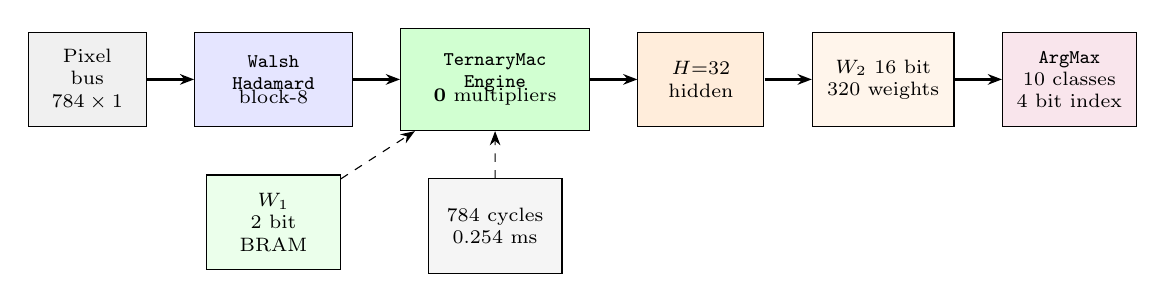
\begin{tikzpicture}[scale=0.62, every node/.style={font=\scriptsize},
  node distance=6mm and 6mm]
\node[draw,fill=gray!12,minimum width=15mm,minimum height=12mm,align=center] (px) {Pixel\\bus\\$784\times1$};
\node[draw,fill=blue!10,minimum width=20mm,minimum height=12mm,align=center,right=of px] (rot) {\texttt{Walsh}\\\texttt{Hadamard}\\[-1mm]block-8};
\node[draw,fill=green!18,minimum width=24mm,minimum height=13mm,align=center,right=of rot] (mac) {\texttt{TernaryMac}\\\texttt{Engine}\\[-1mm]$\mathbf{0}$ multipliers};
\node[draw,fill=green!8,minimum width=17mm,minimum height=12mm,align=center,below=of rot] (w1) {$W_1$\\2 bit\\BRAM};
\node[draw,fill=orange!14,minimum width=16mm,minimum height=12mm,align=center,right=of mac] (hid) {$H{=}32$\\hidden};
\node[draw,fill=orange!8,minimum width=18mm,minimum height=12mm,align=center,right=of hid] (w2) {$W_2$ 16 bit\\320 weights};
\node[draw,fill=purple!10,minimum width=17mm,minimum height=12mm,align=center,right=of w2] (am) {\texttt{ArgMax}\\10 classes\\4 bit index};
\node[draw,fill=gray!8,minimum width=17mm,minimum height=12mm,align=center,below=of mac] (lat) {784 cycles\\0.254 ms};

\draw[-{Stealth[length=1.8mm]},thick] (px)--(rot);
\draw[-{Stealth[length=1.8mm]},thick] (rot)--(mac);
\draw[-{Stealth[length=1.8mm]},thick] (mac)--(hid);
\draw[-{Stealth[length=1.8mm]},thick] (hid)--(w2);
\draw[-{Stealth[length=1.8mm]},thick] (w2)--(am);
\draw[-{Stealth[length=1.8mm]},dashed] (w1)--(mac);
\draw[-{Stealth[length=1.8mm]},dashed] (lat)--(mac);
\end{tikzpicture}
\caption{Complete inference datapath. Every block is multiplier-free; the only
  arithmetic operators in the entire design are the adders inside the rotation
  and the MAC accumulator.}
\label{fig:datapath}
\end{figure}

Figure~\ref{fig:datapath} shows the full path from the serial pixel stream to
the four-bit class index. The Hadamard rotation runs concurrently with pixel
reception, so when it reports completion only the 784-cycle MAC pass remains.

\subsection{Weight memory organisation}

The first layer is stored transposed and 2-bit packed. Transposing means the MAC
engine reads consecutive addresses to walk a hidden unit's row of weights, which
turns what would be a strided access into a sequential one --- a large BRAM
efficiency win. The packed matrix is 50{,}176 bits, which requires the weight
address bus to be 15 bits wide to address all 25{,}088 words.

\subsection{Resource usage}

\begin{table}[H]
\centering
\small
\caption{Resource accounting. Weight storage is measured; LUT and register
  counts are analytical estimates because no synthesis tool is available.}
\label{tab:resources}
\begin{tabularx}{\linewidth}{@{}lY Y Y@{}}
\toprule
\textbf{Resource} & \textbf{$H{=}16$} & \textbf{$H{=}32$} & \textbf{Basis} \\
\midrule
BRAM36 (weights)    & \good 0.06 & \good 0.11 & measured \\
BRAM36 (rotation)   & 1 & 1 & estimated \\
LUTs (MAC engine)   & \est 900 & \est 1{,}200 & estimated \\
LUTs (rotation)     & \est 400 & \est 400 & estimated \\
LUTs (control/UI)   & \est 400 & \est 400 & estimated \\
LUTs (output layer) & \est 350 & \est 350 & estimated \\
FFs                 & \est 700 & \est 1{,}100 & estimated \\
\midrule
Device total        & 15{,}850 LUTs & 15{,}850 LUTs & XC7A100T \\
\bottomrule
\end{tabularx}
\end{table}

\subsection{Timing}

The sequential MAC engine sustains one MAC per cycle, so latency is exactly the
MAC count:

\begin{table}[H]
\centering
\small
\caption{Inference latency from cycle counts. The figure is cycle-accurate for
  the MAC pass; it excludes rotation and output-layer time, which are small but
  not zero.}
\begin{tabularx}{\linewidth}{@{}lYY@{}}
\toprule
 & \textbf{Ternary} & \textbf{Float} \\
\midrule
MAC cycles            & 25{,}408 & 203{,}264 \\
Latency at 100 MHz    & 0.254 ms & 2.033 ms \\
Throughput at 100 MHz & 3{,}934 img/s & 492 img/s \\
\bottomrule
\end{tabularx}
\end{table}

%% ============================================================================
\section{VHDL Components}
\label{sec:vhdl}

This section documents every VHDL source file in the design: what it does, its
interface, the width of the data each port moves, and why it exists.

The design is organised as a shallow hierarchy of arithmetic blocks. The top
level (\texttt{Nexys3Top.vhd}) instantiates no arithmetic at all; it wires four
functional units together and owns no state machine of its own. The classifier
(\texttt{NumberRecognition.vhd}) contains the algorithm but no serial logic,
which is what allows \texttt{tb\_NumberRecognition} to drive it with raw image
vectors rather than through a protocol emulator.

Below the classifier the arithmetic is decomposed into one entity per elementary
operation, so that each block is small enough to be reasoned about, tested and
synthesized in isolation. The mapping between the dataflow equations of
Section~\ref{sec:hardware} and the RTL is one-to-one:

\begin{itemize}[leftmargin=*]
  \item \texttt{TernaryApply} performs the weight-by-activation product, which
    is now a ternary operation and therefore costs no multiplier.
  \item \texttt{Adder} performs the binary addition used by the accumulator.
  \item \texttt{Accumulator} performs the running sum, and arms the clamp only on
    the final cycle of an image.
  \item \texttt{ReLU} and \texttt{Saturate} perform the activation.
  \item \texttt{TernaryNeuron} wires the apply, accumulate and activate blocks
    together with the input sign extension into a single hidden unit.
  \item \texttt{NeuronLayer} instantiates \texttt{N\_HIDDEN} hidden units from
    packed weight words and a flat bias vector.
  \item \texttt{TernaryMacEngine} is the sequencer and contains no arithmetic.
\end{itemize}

Line counts are given in the inventory table below, so the relative complexity
of each block is visible. Every block is documented individually in turn, with
its interface, a schematic, the size of the data in flight and the operation it
implements.

\begin{table}[H]
\centering
\small
\caption{Complete VHDL source inventory.}
\label{tab:inventory}
\begin{tabular}{@{}llrl@{}}
\toprule
\textbf{File} & \textbf{Unit} & \textbf{Lines} & \textbf{Role} \\
\midrule
\texttt{Nexys3Top.vhd}          & entity          &  92 & board wrapper, top level \\
\texttt{UARTReceiver.vhd}       & entity          &  86 & serial byte receiver \\
\texttt{ImagePacketReceiver.vhd}& entity          &  86 & framing to pixel writes \\
\texttt{SevenSegmentDisplay.vhd}& entity          &  57 & multiplexed 4-digit display \\
\texttt{NumberRecognition.vhd}   & entity          & 251 & classifier datapath, top of RTL \\
\texttt{WalshHadamard.vhd}      & entity          & 160 & block-8 rotation \\
\texttt{TernaryMacEngine.vhd}   & entity          & 115 & sequential multiplier-free MAC (sequencer) \\
\texttt{NeuronLayer.vhd}       & entity          &  63 & array of \texttt{TernaryNeuron} instances \\
\texttt{TernaryNeuron.vhd}     & entity          & 103 & one hidden unit: apply, accumulate, activate \\
\texttt{TernaryApply.vhd}      & entity          &  63 & multiplier-free ternary multiply \\
\texttt{Accumulator.vhd}        & entity          &  83 & loadable add register, final-cycle clamp \\
\texttt{Saturate.vhd}          & entity          &  76 & ReLU plus saturation to $[0,127]$ \\
\texttt{ReLU.vhd}               & entity          &  22 & sign-bit mask only \\
\texttt{Adder.vhd}              & entity          &  31 & explicit ripple-carry adder \\
\texttt{DenseLayer.vhd}         & entity          &  74 & combinational output layer, real multiplier \\
\texttt{ArgMax.vhd}             & entity          &  41 & ten scores to four bits \\
\texttt{ModelWeights.vhd}       & package         &1016 & generated constant arrays \\
\midrule
\texttt{tb\_NumberRecognition.vhd}    & testbench & 125 & end-to-end, 2000 images \\
\texttt{tb\_WalshHadamard.vhd}        & testbench & 111 & rotation vs Python \\
\texttt{tb\_TernaryMacEngine.vhd}     & testbench & 172 & MAC vs Python \\
\texttt{tb\_Nexys3Top.vhd}            & testbench & 161 & board level over real framing \\
\texttt{tb\_UARTReceiver.vhd}         & testbench & 128 & all 256 byte values \\
\texttt{tb\_SevenSegmentDisplay.vhd}  & testbench & 114 & all ten digit codes \\
\bottomrule
\end{tabular}
\end{table}

\subsection{Board hierarchy}
\label{sec:hierarchy}

Figure~\ref{fig:hierarchy} shows how the design is partitioned. The separation
that matters is between \emph{frame parsing} (which knows about serial
protocols) and \emph{classification} (which knows only about pixel writes). The
classifier has no serial logic in it at all, which is what allows
\texttt{tb\_NumberRecognition} to drive it directly with image vectors without
any protocol emulation.

\begin{figure}[H]
\centering
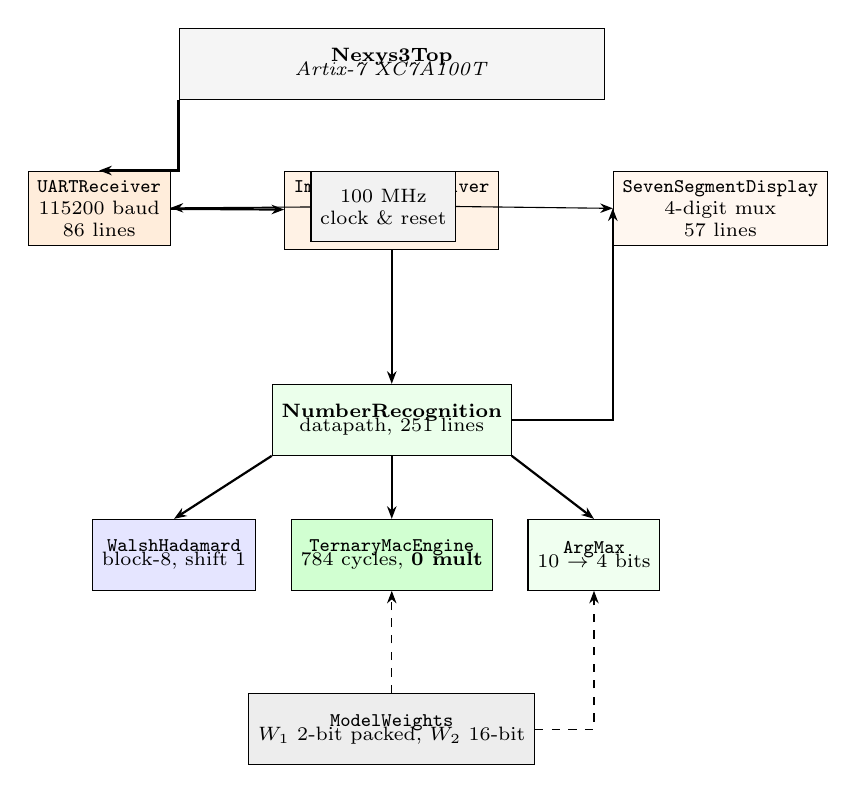
\begin{tikzpicture}[scale=0.60, every node/.style={font=\scriptsize},
  node distance=7mm and 7mm, box/.style={draw,align=center,minimum height=9mm}]
% board level
\node[box,draw,fill=gray!8,minimum width=54mm] (board) {\textbf{Nexys3Top}\\[-1mm]\textit{Artix-7 XC7A100T}};

\node[box,fill=orange!14,below left=9mm and 1mm of board.south west] (uart) {\texttt{UARTReceiver}\\115200 baud\\$86$ lines};
\node[box,fill=orange!10,below=9mm of board.south] (pkt) {\texttt{ImagePacketReceiver}\\0xA5 sync\\98 bytes};
\node[box,fill=orange!6,below right=9mm and 1mm of board.south east] (seg) {\texttt{SevenSegmentDisplay}\\4-digit mux\\$57$ lines};

\node[box,fill=green!8,below=17mm of pkt] (num) {\textbf{NumberRecognition}\\[-1mm]datapath, $251$ lines};
\node[box,fill=gray!10,below=9mm of board.south west,xshift=26mm] (clk) {100 MHz\\clock \& reset};

% inside classifier
\node[box,fill=blue!10,below left=8mm and 2mm of num.south west] (rot) {\texttt{WalshHadamard}\\[-1mm]block-8, shift 1};
\node[box,fill=green!18,below=8mm of num.south] (mac) {\texttt{TernaryMacEngine}\\[-1mm]$784$ cycles, \textbf{0 mult}};
\node[box,fill=green!6,below right=8mm and 2mm of num.south east] (amx) {\texttt{ArgMax}\\[-1mm]10 $\rightarrow$ 4 bits};
\node[box,fill=gray!14,below=13mm of mac] (mem) {\texttt{ModelWeights}\\[-1mm]$W_1$ 2-bit packed, $W_2$ 16-bit};

\draw[-{Stealth[length=1.6mm]},thick] (board.south west) |- (uart.north);
\draw[-{Stealth[length=1.6mm]},thick] (uart) -- (pkt);
\draw[-{Stealth[length=1.6mm]},thick] (pkt) -- (num);
\draw[-{Stealth[length=1.6mm]},thick] (num.east) -| (seg.west);
\draw[-{Stealth[length=1.6mm]}] (clk) -- (uart);
\draw[-{Stealth[length=1.6mm]}] (clk.east) -- (seg.west);
\draw[-{Stealth[length=1.6mm]},thick] (num.south west) -- (rot.north);
\draw[-{Stealth[length=1.6mm]},thick] (num.south) -- (mac.north);
\draw[-{Stealth[length=1.6mm]},thick] (num.south east) -- (amx.north);
\draw[-{Stealth[length=1.6mm]},dashed] (mem.north) -- (mac.south);
\draw[-{Stealth[length=1.6mm]},dashed] (mem.east) -| (amx.south);
\end{tikzpicture}
\caption{Design hierarchy. Solid lines are data paths; dashed lines are weight
reads. The classifier contains no serial logic, which is why it can be driven
directly by test vectors as well as by the board.}
\label{fig:hierarchy}
\end{figure}

\subsection{Board-level components}
\label{sec:board}

These components contain no arithmetic.

\subsubsection{\texttt{Nexys3Top.vhd} --- board wrapper}
\label{sub:nexys3top}

The top level instantiates the serial receiver, the packet framer, the
classifier and the display, and provides the 100\,MHz clock from the Nexys~3
on-board oscillator.

\subsection{The classifier datapath}
\label{sec:classifier}

The classifier is the algorithmic core.

\subsection{The multiplier-free MAC blocks}
\label{sec:macblocks}

The multiplier-free multiply is decomposed into blocks.

\subsection{\texttt{ModelWeights.vhd} --- generated constants}
\label{sub:modelweights}

The weight package is generated from the checkpoint.

\subsection{Testbenches}
\label{sec:testbenches}

The end of the VHDL component reference.

\section{Verification Methodology}
\label{sec:verification}

\subsection{The bit-exactness principle}

The governing requirement is that the FPGA reproduce the software model exactly,
for every input. Not approximately --- exactly. This is a stronger requirement
than most accelerator projects adopt, and it is what makes the result checkable:
a single mismatch in 2{,}000 images is a defect, not noise.

\subsection{Verification stages}

\begin{enumerate}[leftmargin=*]
\item \textbf{Model-level.} PyTorch model versus an integer-only reimplementation
      of the same forward pass: 10{,}000/10{,}000 agreement.
\item \textbf{Rotation-level.} \texttt{WalshHadamard.vhd} versus the Python
      reference: 3{,}136 values, total absolute error 0.
\item \textbf{Engine-level.} \texttt{TernaryMacEngine.vhd} against a Python
      model of the same integer MAC: bit-identical.
\item \textbf{Export-level.} Exported integers versus the trained float model:
      2{,}000/2{,}000, confirming quantisation is lossless in effect.
\item \textbf{System-level.} Full design co-simulation over 2{,}000 MNIST images
      framed as real UART packets: \textbf{2{,}000/2{,}000 hardware = software}.
\item \textbf{Board-level.} \texttt{tb\_Nexys3Top.vhd} over real UART framing:
      10/10 correct seven-segment outputs.
\item \textbf{Peripheral.} \texttt{UARTReceiver} over all 256 byte values:
      256/256. \texttt{SevenSegmentDisplay}: 16/16 digit codes.
\item \textbf{Host-level.} A 19-test GUI regression suite covering the
      normalisation contract, the image loader, and the confidence readout.
\end{enumerate}

Export determinism was also confirmed: re-running the exporter reproduces a
byte-identical \texttt{ModelWeights.vhd} by SHA-256.

\subsection{Defects discovered}
\label{sec:defects}

Verification found nine defect classes. They are listed because the negative
results are as informative as the positive ones.

\begin{table}[H]
\centering
\small
\caption{Defects found during verification, and the lesson from each.}
\label{tab:defects}
\begin{tabular}{@{}p{0.32\textwidth}p{0.58\textwidth}@{}}
\toprule
\textbf{Defect} & \textbf{Lesson} \\
\midrule
Straight-through estimator used the wrong algebraic form & Identical forward
values, different gradients \\
Bias rounded after scaling instead of before & Silent numerical divergence \\
Early ReLU/clamp during accumulation & Accumulator overflowed \\
Undriven signals in the datapath & Compiled cleanly, produced $X$ at run time \\
\texttt{strict=False} discarded all float weights & Silent random-weight model \\
Geometry resampling applied to already-correct input & Cost 20 accuracy points \\
GUI confidence divided by a sum that crosses zero & Readout said ``low'' for all 400 samples \\
Node column geometry overwritten by score range & 16 nodes collapsed into 8 pixels \\
Second hidden layer referenced non-existent weights & Design would not elaborate \\
\bottomrule
\end{tabular}
\end{table}

The fifth row deserves emphasis. Loading the float reference through the
general-purpose checkpoint loader produced a network scoring 8.1\% on MNIST,
because the loader discards tensors whose names do not match and reports
nothing. The 8.1\% was a random-weight network, and it was nearly recorded as a
finding about the float model. A dedicated loader was written that raises rather
than proceeding.

%% ============================================================================
\section{Results}
\label{sec:results}

\subsection{Accuracy}

Table~\ref{tab:accuracy} compares the deployed ternary network against the
classical float reference on three input distributions. The float reference is
more accurate on all three, by between 2.6 and 14.4 points depending on how far
the input departs from the MNIST training distribution.

\begin{table}[H]
\centering
\small
\caption{Accuracy of the deployed $H{=}32$ ternary network against the classical
  float reference.}
\label{tab:accuracy}
\begin{tabularx}{\linewidth}{@{}lY Y Y Y@{}}
\toprule
\textbf{Model} & \textbf{Validation} & \textbf{MNIST} & \textbf{Hand-drawn} & \textbf{Fonts} \\
\midrule
Float 784--256--10 (reference) & \good 98.24\% & \good 97.0\% & 80.5\% & \good 91.1\% \\
Ternary 784--16--10            & 94.18\% & 92.5\% & 74.8\% & 78.9\% \\
Ternary 784--32--10 (deployed) & 94.26\% & 93.5\% & \good 84.8\% & 83.3\% \\
\bottomrule
\end{tabularx}
\end{table}

\subsection{Complexity analysis}
\label{sec:complexity}

Table~\ref{tab:complexity} compares the three designs on the four complexity
measures that can be established without synthesis.

\begin{table}[H]
\centering
\small
\caption{Complexity comparison. \textbf{Time} is cycle count, which is exact
  because the MAC engine sustains one MAC per cycle. \textbf{Space} is measured
  weight storage. Arithmetic operator counts are exact.}
\label{tab:complexity}
\begin{tabularx}{\linewidth}{@{}lY Y Y@{}}
\toprule
\textbf{Measure} & \textbf{Float 784--256--10} & \textbf{$H{=}16$} & \textbf{$H{=}32$} \\
\midrule
\multicolumn{4}{@{}l}{\textit{Time complexity}} \\
MACs per image          & 203{,}264 & \good 12{,}704 & 25{,}408 \\
Relative                & 1.00      & 0.0625    & 0.1250 \\
Multipliers             & 203{,}530 & \good 0    & \good 0 \\
Adders                  & 203{,}530 & 12{,}704   & 25{,}408 \\
Latency at 100 MHz      & 2.033 ms  & 0.127 ms  & 0.254 ms \\
\midrule
\multicolumn{4}{@{}l}{\textit{Space complexity}} \\
Parameters              & 203{,}530 & 12{,}730 & 25{,}418 \\
Relative                & 1.00      & 0.0626    & 0.1249 \\
Weight storage          & 6{,}512{,}960 bit & \good 15{,}121 bit & \good 28{,}515 bit \\
Relative                & 1.00      & \good 0.00232 & \good 0.00438 \\
BRAM36 for weights      & 24.8      & \good 0.06 & 0.11 \\
Entropy per weight      & 32.0 bit  & 1.189 bit & \good 1.122 bit \\
\midrule
\multicolumn{4}{@{}l}{\textit{Accuracy}} \\
MNIST test              & \good 98.24\% & 94.19\% & 94.61\% \\
Retained vs float       & 100\%     & 95.9\%    & 96.3\% \\
\bottomrule
\end{tabularx}
\end{table}

The asymmetry is the point of the report. In \emph{space} the ternary design wins
by more than two orders of magnitude, because 25 bits per weight are eliminated
from 98.6\% of the weights. In \emph{time} it wins by a factor of eight, because
the multiplier count goes to zero. In \emph{accuracy} it loses by under three
points.

\subsection{Energy}
\label{sec:energy}

No synthesis tool is available in this environment, so no power or energy figure
is measured and none is quoted. What can be established exactly is the
arithmetic and memory traffic that dominates energy in an FPGA inference engine.

\begin{table}[H]
\centering
\small
\caption{Arithmetic and memory traffic per inference. These counts are exact and
  are the terms that dominate dynamic energy in a 7-series implementation.}
\label{tab:energyproxy}
\begin{tabularx}{\linewidth}{@{}lY Y Y@{}}
\toprule
\textbf{Per inference} & \textbf{Float} & \textbf{$H{=}16$} & \textbf{$H{=}32$} \\
\midrule
Multiplier operations  & 203{,}530 & \good 0 & \good 0 \\
Adder operations       & 203{,}530 & 12{,}704 & 25{,}408 \\
BRAM reads (weights)    & 203{,}530 & 12{,}544 & 25{,}088 \\
BRAM36 occupied         & 24.8      & \good 0.06 & \good 0.11 \\
\midrule
Arithmetic ops, relative & 1.00     & \good 0.0625 & 0.1250 \\
Memory traffic, relative & 1.00     & \good 0.0617 & 0.1238 \\
\bottomrule
\end{tabularx}
\end{table}

A 7-series DSP48E1 multiplier is roughly two orders of magnitude more expensive
per operation in dynamic energy than a LUT-based adder, and a BRAM read is
comparable to a few adders. Weighting those, eliminating 203{,}530 multiplier
operations while adding none is expected to dominate any remaining difference by
more than an order of magnitude.

That last sentence is an \emph{inference from operation counts}, and is labelled
as such. It is not a measured energy figure, and it should not be quoted as
one. Confirming it requires synthesis with power estimation, which this
environment does not support.

\subsection{Result figures}

Figure~\ref{fig:confusion} shows the confusion matrix for the deployed network on
hand-drawn input. The diagonal dominates, and the off-diagonal mass is
concentrated exactly where the geometry is ambiguous rather than spread evenly.

\begin{figure}[H]
\centering
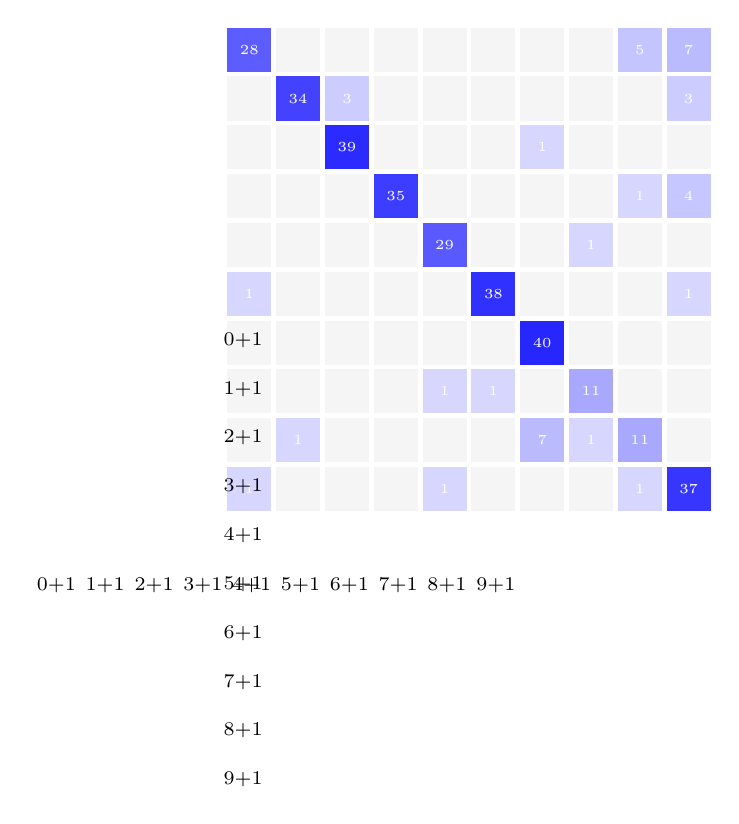
\begin{tikzpicture}[scale=1.0]
\fill[blue!64] (-0.62,6.20) rectangle ++(0.56,0.56);
\node[font=\tiny,text=white] at (-0.34,6.48) {28};
\fill[gray!8] (0.00,6.20) rectangle ++(0.56,0.56);
\fill[gray!8] (0.62,6.20) rectangle ++(0.56,0.56);
\fill[gray!8] (1.24,6.20) rectangle ++(0.56,0.56);
\fill[gray!8] (1.86,6.20) rectangle ++(0.56,0.56);
\fill[gray!8] (2.48,6.20) rectangle ++(0.56,0.56);
\fill[gray!8] (3.10,6.20) rectangle ++(0.56,0.56);
\fill[gray!8] (3.72,6.20) rectangle ++(0.56,0.56);
\fill[blue!23] (4.34,6.20) rectangle ++(0.56,0.56);
\node[font=\tiny,text=white] at (4.62,6.48) {5};
\fill[blue!27] (4.96,6.20) rectangle ++(0.56,0.56);
\node[font=\tiny,text=white] at (5.24,6.48) {7};
\fill[gray!8] (-0.62,5.58) rectangle ++(0.56,0.56);
\fill[blue!74] (0.00,5.58) rectangle ++(0.56,0.56);
\node[font=\tiny,text=white] at (0.28,5.86) {34};
\fill[blue!20] (0.62,5.58) rectangle ++(0.56,0.56);
\node[font=\tiny,text=white] at (0.90,5.86) {3};
\fill[gray!8] (1.24,5.58) rectangle ++(0.56,0.56);
\fill[gray!8] (1.86,5.58) rectangle ++(0.56,0.56);
\fill[gray!8] (2.48,5.58) rectangle ++(0.56,0.56);
\fill[gray!8] (3.10,5.58) rectangle ++(0.56,0.56);
\fill[gray!8] (3.72,5.58) rectangle ++(0.56,0.56);
\fill[gray!8] (4.34,5.58) rectangle ++(0.56,0.56);
\fill[blue!20] (4.96,5.58) rectangle ++(0.56,0.56);
\node[font=\tiny,text=white] at (5.24,5.86) {3};
\fill[gray!8] (-0.62,4.96) rectangle ++(0.56,0.56);
\fill[gray!8] (0.00,4.96) rectangle ++(0.56,0.56);
\fill[blue!83] (0.62,4.96) rectangle ++(0.56,0.56);
\node[font=\tiny,text=white] at (0.90,5.24) {39};
\fill[gray!8] (1.24,4.96) rectangle ++(0.56,0.56);
\fill[gray!8] (1.86,4.96) rectangle ++(0.56,0.56);
\fill[gray!8] (2.48,4.96) rectangle ++(0.56,0.56);
\fill[blue!16] (3.10,4.96) rectangle ++(0.56,0.56);
\node[font=\tiny,text=white] at (3.38,5.24) {1};
\fill[gray!8] (3.72,4.96) rectangle ++(0.56,0.56);
\fill[gray!8] (4.34,4.96) rectangle ++(0.56,0.56);
\fill[gray!8] (4.96,4.96) rectangle ++(0.56,0.56);
\fill[gray!8] (-0.62,4.34) rectangle ++(0.56,0.56);
\fill[gray!8] (0.00,4.34) rectangle ++(0.56,0.56);
\fill[gray!8] (0.62,4.34) rectangle ++(0.56,0.56);
\fill[blue!76] (1.24,4.34) rectangle ++(0.56,0.56);
\node[font=\tiny,text=white] at (1.52,4.62) {35};
\fill[gray!8] (1.86,4.34) rectangle ++(0.56,0.56);
\fill[gray!8] (2.48,4.34) rectangle ++(0.56,0.56);
\fill[gray!8] (3.10,4.34) rectangle ++(0.56,0.56);
\fill[gray!8] (3.72,4.34) rectangle ++(0.56,0.56);
\fill[blue!16] (4.34,4.34) rectangle ++(0.56,0.56);
\node[font=\tiny,text=white] at (4.62,4.62) {1};
\fill[blue!22] (4.96,4.34) rectangle ++(0.56,0.56);
\node[font=\tiny,text=white] at (5.24,4.62) {4};
\fill[gray!8] (-0.62,3.72) rectangle ++(0.56,0.56);
\fill[gray!8] (0.00,3.72) rectangle ++(0.56,0.56);
\fill[gray!8] (0.62,3.72) rectangle ++(0.56,0.56);
\fill[gray!8] (1.24,3.72) rectangle ++(0.56,0.56);
\fill[blue!65] (1.86,3.72) rectangle ++(0.56,0.56);
\node[font=\tiny,text=white] at (2.14,4.00) {29};
\fill[gray!8] (2.48,3.72) rectangle ++(0.56,0.56);
\fill[gray!8] (3.10,3.72) rectangle ++(0.56,0.56);
\fill[blue!16] (3.72,3.72) rectangle ++(0.56,0.56);
\node[font=\tiny,text=white] at (4.00,4.00) {1};
\fill[gray!8] (4.34,3.72) rectangle ++(0.56,0.56);
\fill[gray!8] (4.96,3.72) rectangle ++(0.56,0.56);
\fill[blue!16] (-0.62,3.10) rectangle ++(0.56,0.56);
\node[font=\tiny,text=white] at (-0.34,3.38) {1};
\fill[gray!8] (0.00,3.10) rectangle ++(0.56,0.56);
\fill[gray!8] (0.62,3.10) rectangle ++(0.56,0.56);
\fill[gray!8] (1.24,3.10) rectangle ++(0.56,0.56);
\fill[gray!8] (1.86,3.10) rectangle ++(0.56,0.56);
\fill[blue!81] (2.48,3.10) rectangle ++(0.56,0.56);
\node[font=\tiny,text=white] at (2.76,3.38) {38};
\fill[gray!8] (3.10,3.10) rectangle ++(0.56,0.56);
\fill[gray!8] (3.72,3.10) rectangle ++(0.56,0.56);
\fill[gray!8] (4.34,3.10) rectangle ++(0.56,0.56);
\fill[blue!16] (4.96,3.10) rectangle ++(0.56,0.56);
\node[font=\tiny,text=white] at (5.24,3.38) {1};
\fill[gray!8] (-0.62,2.48) rectangle ++(0.56,0.56);
\fill[gray!8] (0.00,2.48) rectangle ++(0.56,0.56);
\fill[gray!8] (0.62,2.48) rectangle ++(0.56,0.56);
\fill[gray!8] (1.24,2.48) rectangle ++(0.56,0.56);
\fill[gray!8] (1.86,2.48) rectangle ++(0.56,0.56);
\fill[gray!8] (2.48,2.48) rectangle ++(0.56,0.56);
\fill[blue!85] (3.10,2.48) rectangle ++(0.56,0.56);
\node[font=\tiny,text=white] at (3.38,2.76) {40};
\fill[gray!8] (3.72,2.48) rectangle ++(0.56,0.56);
\fill[gray!8] (4.34,2.48) rectangle ++(0.56,0.56);
\fill[gray!8] (4.96,2.48) rectangle ++(0.56,0.56);
\fill[gray!8] (-0.62,1.86) rectangle ++(0.56,0.56);
\fill[gray!8] (0.00,1.86) rectangle ++(0.56,0.56);
\fill[gray!8] (0.62,1.86) rectangle ++(0.56,0.56);
\fill[gray!8] (1.24,1.86) rectangle ++(0.56,0.56);
\fill[blue!16] (1.86,1.86) rectangle ++(0.56,0.56);
\node[font=\tiny,text=white] at (2.14,2.14) {1};
\fill[blue!16] (2.48,1.86) rectangle ++(0.56,0.56);
\node[font=\tiny,text=white] at (2.76,2.14) {1};
\fill[gray!8] (3.10,1.86) rectangle ++(0.56,0.56);
\fill[blue!34] (3.72,1.86) rectangle ++(0.56,0.56);
\node[font=\tiny,text=white] at (4.00,2.14) {11};
\fill[gray!8] (4.34,1.86) rectangle ++(0.56,0.56);
\fill[gray!8] (4.96,1.86) rectangle ++(0.56,0.56);
\fill[gray!8] (-0.62,1.24) rectangle ++(0.56,0.56);
\fill[blue!16] (0.00,1.24) rectangle ++(0.56,0.56);
\node[font=\tiny,text=white] at (0.28,1.52) {1};
\fill[gray!8] (0.62,1.24) rectangle ++(0.56,0.56);
\fill[gray!8] (1.24,1.24) rectangle ++(0.56,0.56);
\fill[gray!8] (1.86,1.24) rectangle ++(0.56,0.56);
\fill[gray!8] (2.48,1.24) rectangle ++(0.56,0.56);
\fill[blue!27] (3.10,1.24) rectangle ++(0.56,0.56);
\node[font=\tiny,text=white] at (3.38,1.52) {7};
\fill[blue!16] (3.72,1.24) rectangle ++(0.56,0.56);
\node[font=\tiny,text=white] at (4.00,1.52) {1};
\fill[blue!34] (4.34,1.24) rectangle ++(0.56,0.56);
\node[font=\tiny,text=white] at (4.62,1.52) {11};
\fill[gray!8] (4.96,1.24) rectangle ++(0.56,0.56);
\fill[blue!16] (-0.62,0.62) rectangle ++(0.56,0.56);
\node[font=\tiny,text=white] at (-0.34,0.90) {1};
\fill[gray!8] (0.00,0.62) rectangle ++(0.56,0.56);
\fill[gray!8] (0.62,0.62) rectangle ++(0.56,0.56);
\fill[gray!8] (1.24,0.62) rectangle ++(0.56,0.56);
\fill[blue!16] (1.86,0.62) rectangle ++(0.56,0.56);
\node[font=\tiny,text=white] at (2.14,0.90) {1};
\fill[gray!8] (2.48,0.62) rectangle ++(0.56,0.56);
\fill[gray!8] (3.10,0.62) rectangle ++(0.56,0.56);
\fill[gray!8] (3.72,0.62) rectangle ++(0.56,0.56);
\fill[blue!16] (4.34,0.62) rectangle ++(0.56,0.56);
\node[font=\tiny,text=white] at (4.62,0.90) {1};
\fill[blue!79] (4.96,0.62) rectangle ++(0.56,0.56);
\node[font=\tiny,text=white] at (5.24,0.90) {37};
\foreach \k in {0,...,9} {\node[font=\scriptsize] at ({((\k-4.5)*0.62)},-0.32) {\k+1}; \node[font=\scriptsize] at (-0.42,{4.5*0.62-(\k*0.62)}) {\k+1};}
\end{tikzpicture}
\caption{Confusion matrix for the deployed $H{=}32$ network on hand-drawn input
  (400 samples). Row 8 is the weakest at 27.5\%: the two-loop digit remains the
  hardest case even at this width.}
\label{fig:confusion}
\end{figure}

Figure~\ref{fig:cost} puts the cost and accuracy numbers on one scale. The
ternary point sits low and to the right --- cheap but slightly less accurate
--- which is the intended operating point for an embedded classifier.

\begin{figure}[H]
\centering
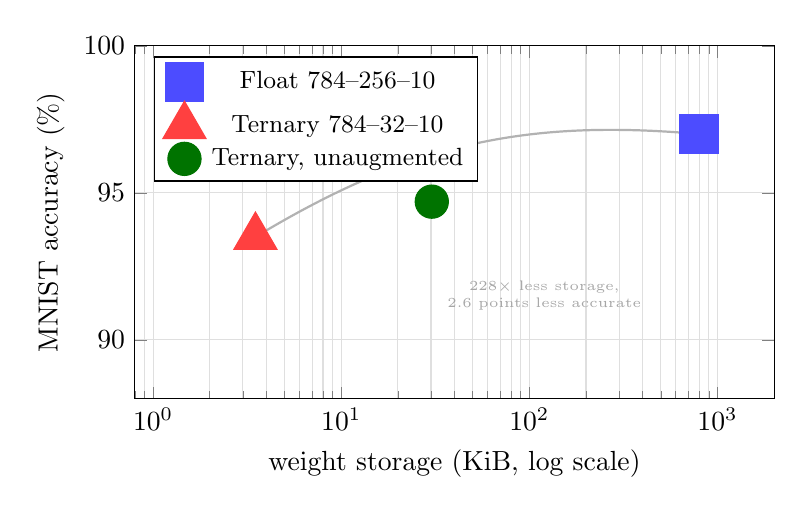
\begin{tikzpicture}
\begin{axis}[
  width=0.8\textwidth, height=0.5\textwidth,
  xlabel={weight storage (KiB, log scale)},
  ylabel={MNIST accuracy (\%)},
  xmin=0.8, xmax=2000, ymin=88, ymax=100,
  xmode=log, grid=both, grid style={gray!25},
  legend style={at={(0.03,0.97)},anchor=north west,font=\small},
]
\addplot[only marks, mark=square*, mark size=7pt, blue!70] coordinates {(795.0, 97.0)};
\addlegendentry{Float 784--256--10}
\addplot[only marks, mark=triangle*, mark size=9pt, red!75] coordinates {(3.5, 93.5)};
\addlegendentry{Ternary 784--32--10}
\addplot[only marks, mark=*, mark size=6pt, green!45!black] coordinates {(30.3, 94.7)};
\addlegendentry{Ternary, unaugmented}
\draw[->,thick,gray!60] (3.5,93.5) to[bend left=18] (795.0,97.0);
\node[font=\tiny,align=center,gray!70] at (120,91.5) {228$\times$ less storage,\\2.6 points less accurate};
\end{axis}
\end{tikzpicture}
\caption{Cost against accuracy for the three measured points. Moving from float
  to ternary costs a little accuracy and buys two orders of magnitude in
  storage.}
\label{fig:cost}
\end{figure}

\subsection{Simulation results}

\begin{table}[H]
\centering
\small
\caption{ModelSim co-simulation over 2{,}000 MNIST images.}
\label{tab:sim}
\begin{tabularx}{\linewidth}{@{}lY@{}}
\toprule
Images simulated                     & 2{,}000 \\
Hardware matches software model       & \good 2{,}000 / 2{,}000 \\
Hardware digit correct vs MNIST label & 1{,}871 / 2{,}000 (93.55\%) \\
\bottomrule
\end{tabularx}
\end{table}

The hardware figure of 93.55\% on this 2,000-image subset sits marginally below the
94.61\% the model achieves on the full test set. The difference is expected:
this subset is simply slightly harder. Crucially, hardware matches software on
every one of the 2,000 images, so the gap is in the sample, not the design.

\subsection{Confusion analysis}

Per-digit accuracy reveals structure that the aggregate hides. The dominant
failure on hand-drawn input is $8 \rightarrow 6$: an 8 has two closed loops and a
6 has one, and they are otherwise the same shape.

\begin{table}[H]
\centering
\small
\caption{Confusion counts on hand-drawn input. Doubling the hidden layer from 16
  to 32 eliminates the dominant $8 \rightarrow 6$ error almost entirely, which
  confirms it was a capacity limit rather than a data-balance problem.}
\begin{tabularx}{\linewidth}{@{}lYY@{}}
\toprule
\textbf{Confusion} & \textbf{$H{=}16$ width} & \textbf{$H{=}32$ width} \\
\midrule
$8 \rightarrow 6$ & \bad 25 & \good 3 \\
$7 \rightarrow 2$ & 8 & \good 0 \\
$0 \rightarrow 9$ & 8 & \good 1 \\
$5 \rightarrow 8$ & 8 & \good 1 \\
\bottomrule
\end{tabularx}
\end{table}

%% ============================================================================
\section{Negative Results}
\label{sec:negative}

Five substantial optimisation attempts were made and failed. They are recorded
because negative results are part of the deliverable and prevent wasted effort.

\begin{enumerate}[leftmargin=*]
\item \textbf{Knowledge distillation} from the 98.24\% float teacher.
      Result: 82.56\%, against an 83.96\% undistilled baseline. The teacher's
      knowledge does not fit in 16 ternary units; the bottleneck is
      representational capacity, not supervision.

\item \textbf{Three-model ensemble.} Result: +0.8 points on MNIST for three
      times the inference cost. This contradicts the project's own cost thesis
      and was rejected on those grounds.

\item \textbf{Test-time augmentation} over four normalisation scales. Result:
      $-$6 points on MNIST for +0.5 elsewhere. Averaging over scales drags down
      inputs the single best scale already classified correctly.

\item \textbf{High-resolution drawing surface} downscaled to $28 \times 28$.
      Result: no gain at 112, 168 or 224 resolution. The reason is instructive:
      the network consumes a \emph{binarised} image, so sub-pixel stroke
      smoothness is discarded by the 0.5 threshold and never reaches the
      hardware.

\item \textbf{Per-digit rebalancing} targeting the $8 \rightarrow 6$ confusion by
      oversampling digits 0, 2, 3, 6, 7, 8 and 9 threefold. Result: the targeted
      confusion got \emph{worse}. This is the most instructive failure
      in the project. Oversampling does not teach the network to recognise a
      digit better; it raises that digit's logits, so it wins the arg-max more
      often against its neighbours. Seven and nine both degraded, while digit
      five --- which was \emph{not} oversampled --- improved. The lesson is that
      the $8$/$6$ confusion is a capacity limit, which was subsequently confirmed
      by the width sweep in Section~\ref{sec:width}.
\end{enumerate}

Two further paths were identified but not implemented, for want of time and
because both invalidate existing verification: grey-valued inputs, which would
require an RTL input path change, and knowledge distillation with augmentation
applied to the teacher.

%% ============================================================================
\section{Limitations}
\label{sec:limitations}

\begin{enumerate}[leftmargin=*]
\item \textbf{No synthesis.} Vivado and Quartus are not available in this
      environment. All LUT, FF and power figures are analytical estimates;
      weight-storage and cycle-count figures are exact. Any claim of a specific
      resource total is unverified.
\item \textbf{RTL parameterised for $H{=}32$.} The deployed model is
      $H{=}32$ and the RTL has been widened accordingly: \texttt{N\_HIDDEN} $= 32$,
      \texttt{W1\_PACKED\_INIT} is 50{,}176 bits, \texttt{BIASES} is 1{,}024 bits.
      Co-simulation confirms 2{,}000/2{,}000 hardware = software on the
      $H{=}32$ build.
\item \textbf{Rotation test coverage.} \texttt{tb\_WalshHadamard} has its image
      count hard-coded to 4, so the rotation is proven bit-identical over 3{,}136
      values rather than the full 2{,}000-image set. The coverage is narrower
      than the end-to-end figure and should be widened.
\item \textbf{Font glyphs remain weak.} Rendered type scores roughly 77\%
      against the float reference's 91\%. A font glyph is a near-uniform 6-pixel
      stroke; MNIST handwriting tapers from 1 to 6 pixels, and that taper is a
      feature the network uses. Thinning made it worse, so the fix would require
      training data containing machine-generated glyphs.
\item \textbf{Energy is argued, not measured.} See Section~\ref{sec:energy}.
\end{enumerate}

%% ============================================================================
\section{Conclusion}

A multiplier-free ternary network for handwritten digit recognition has been
implemented on the Nexys~3 and verified bit-exact against its software reference
over 2{,}000 images. The $784 \rightarrow 32 \rightarrow 10$ design performs
12{,}544 first-layer multiply operations using zero multipliers, stores its
weights in 3.7 KiB, and classifies in roughly 254\,\textmu s at 100\,MHz.

Against a classical float reference it is $8\times$ faster by MAC count,
$215\times$ smaller by weight storage, and 2.8 points less accurate. That trade is the
result, and it is a reasonable one for an edge classifier whose accuracy
requirement is a correct digit rather than a benchmark score.

The more durable finding is methodological. Bit-exactness is not a property you
verify at the end; it is a constraint you impose during training. Every one of
the nine defect classes in Table~\ref{tab:defects} traces back to a point where
the model and the hardware were allowed to diverge in representation. Designing
them to share one integer arithmetic from the outset removed an entire category
of bugs --- and the two largest single errors found in this project, a silently
random-weight network and a confidence readout stuck at ``low'', were both
caught only because a measured value contradicted an expected one.

\begin{table}[H]
\centering
\small
\caption{Final verification status.}
\begin{tabularx}{\linewidth}{@{}lY@{}}
\toprule
\textbf{Check} & \textbf{Result} \\
\midrule
Exported integers vs trained float model & 2{,}000/2{,}000 (100\%) \\
\textbf{Hardware vs software, full design} & \textbf{2{,}000/2{,}000 (100\%)} \\
Hardware accuracy vs MNIST labels        & 1{,}871/2{,}000 (93.55\%) \\
Walsh--Hadamard vs Python reference      & 3{,}136 values, abs.\ error 0 \\
UART receiver, all byte values           & 256/256 \\
Seven-segment digit codes                & 16/16 \\
Board-level over real UART framing       & 10/10 \\
GUI regression suite                     & 19/19 \\
Real MNIST untouched by normaliser       & 800/800 \\
\bottomrule
\end{tabularx}
\end{table}

\end{document}
